\chapter{Computer Methods and Results}
\label{ch:computer-results}

In order to guide our investigation of the levelability of graphs, we used computational tools to check for the existence of valid solutions to \autoref{thm:level-condition} on graphs on small numbers of vertices. In particular, a computer script was written using SageMath to check all connected graphs on 10 or fewer vertices.

\section{Data generation}
Using the convenient built-in capabilities of SageMath, we applied \autoref{thm:level-condition} to determine levelability on all connected graphs on 10 or fewer vertices. Graphs were generated using the \texttt{graphs.nauty\_geng()} generator object in SageMath. The $t$ maximal independent sets for each graph \texttt{G} were extracted using the function \texttt{IndependentSets(G, maximal = True)}, and the corresponding linear system was constructed as a matrix with $t-1$ rows and $n$ columns. The existence of integer solutions to \autoref{thm:level-condition} with the $x_i \geq 2$ constraint were checked using \texttt{MixedIntegerLinearProgram()}: a built-in linear program function in SageMath. The solution to the system, if one was returned by the linear program, was checked against the original system to verify the solution. If the linear program failed to return a solution, the graph was determined to not be levelable. 

One challenge in recording these data is that graphs do not have unique vertex labellings. Therefore, the graph object generated by \texttt{graphs.nauty\_geng()} may not be the same ``object" as an isomorphic, but differently labelled graph. Therefore, before recording data, each generated graph object was transformed to a unique ``canonical" label using \texttt{canonical\_label()}. If we were to then generate an isomorphism of some graph in another analysis, we can reduce it to the canonical label to match our data set to avoid miscommunication and confusion. The graph6 string for each (canonically labelled) graph was saved in a data frame along with a boolean variable (\texttt{1} if levelable or \texttt{0} if not). The source code and data for this project is available at \url{https://github.com/michael-chong/levelable}. Psuedocode for the data generation is outlined in  \autoref{lst:pseudocode}.

\begin{lstlisting}[mathescape = true, float=bthp,frame=tb,caption={Data generation pseudocode},label=lst:pseudocode]
for n = 4,...,10:
  
  DF = data frame to hold results
  
  for each connected graph G on n vertices:
    G := canonical labelling of G
    g6string := graph6 string of G
    F := list of maximal independent sets of G
    t := length of F (number of facets)
    A := zero matrix with (t-1) rows and n columns 
    b := column vector with (t-1) rows
    
    for i = 1,...,t-1:
      for each vertex v in the ith facet:
        set A[i, v] = 1
        set b[i] = b[i] + 1
      for each vertex v in the (i+1)th facet:
      	set A[i+1, v] = A[i+1, v] - 1
        set b[i] = b[i] - 1
    
    x := new (vector) variable for linear program
    for k = 1,...,n:
    	set constraint {x[k] $\geq$ 2}
    for i = 1, ...., t-1:
    	for k = 1,...,n:
          set constraint {A[i,k]*x[k] = b[i]}
   
    if a valid solution x can be found by the linear program:
        append to DF: {g6string, levelable = 1}
    if no valid solution x can be found by the linear program:
        append to DF: {g6string, levelable = 0}
\end{lstlisting}

\section{Enumeration of levelable graphs} \label{sec:enumeration}
The data generated gives us the number of connected, levelable graphs on 10 or fewer vertices. These results are given in \autoref{tab:enumeration}. 

\begin{table}[bth]
    \myfloatalign
    \begin{tabularx}{\textwidth}{@{}r *5{>{\centering\arraybackslash}X}@{}} %the weird stuff is for centering
    	\toprule
        \tableheadline{$n$} & \tableheadline{connected} & \tableheadline{levelable} & \tableheadline{well-covered \cite{Baker2016}} & \tableheadline{Cohen-Macaulay\cite{Baker2016}}\\ 
        \midrule
        5	& 	21			&	20 			&	6		&	5	\\
        6 	&	112			&	97			&	27		&	20	\\
        7	&	853			&	619			&	108		&	82	\\
        8	&	11 117		&	6001		&	788		&	565	\\
        9	&	261 080		&	90 346		&	9035	&	5688	\\
    	10	&	11 716 571	&	1 364 609	&	196 928	&	102 035	\\
        \bottomrule
    \end{tabularx}
    \caption{Enumeration of connected levelable graphs on $n$ vertices. Results from \cite{Baker2016} enumerating well-covered and Cohen-Macaulay graphs are also given for comparison.}  \label{tab:enumeration}
\end{table}

We remark that the proportion of levelable graphs seems to decrease dramatically as $n$ increases past 9 vertices. However it remains an open question of how many graphs on $n$ vertices are levelable in general. In \autoref{ch:non-levelable-results}, we discuss criteria for graphs which fail to be levelable, which provides some insight into the scarcity of levelable graphs on large numbers of graphs. 

Furthermore, our data is consistent with computations from \cite{Baker2016}. From \autoref{thm:pure}, we know that the independence complexes of well-covered graphs are pure and therefore all such graphs are levelable. We would therefore expect that the levelable graphs are a superset of the set of well-covered graphs, and \autoref{tab:enumeration} shows this is indeed the case.

\section{Smallest non-levelable graph} \label{sec:smallest}

Theorem 11 in \cite{VanTuyl2010} states that for every $n \geq 5$, there exists a simplicial complex on $n$ vertices which is not levelable. However, it is unclear whether this is true for independence complexes of graphs, and prior to this investigation, a minimal example of an independence complex that fails to be levelable had not yet been found. Our computational search revealed that the smallest example of a non-levelable graph is the path on 5 vertices. We can verify this result by showing there cannot exist a valid solution to \autoref{thm:level-condition}.
\begin{figure}[bth]
    \myfloatalign
    \vspace{0.5cm}
    {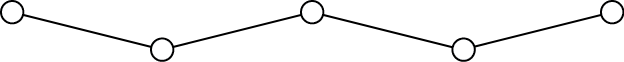
\includegraphics[width=.55\linewidth]{figures/5-path.png}} 
    \vspace{0.5cm}
    \caption{The path graph on 5 vertices. This is the smallest example of a graph that is not levelable.}
\end{figure}

\begin{example} \label{ex:5-path}
Let $P$ denote the path on 5 vertices $V(P) = \br{v_1, \dots, v_5}$, and edge set $E(G) = \br{\br{v_i, v_{i+1} \; | \; i = 1, \dots, 4}}$. Then 
\begin{equation*}
\begin{aligned}
F_1 &= \br{v_1, v_3, v_5}, \\
F_2 &= \br{v_2, v_4} \\
F_3 &= \br{v_1, v_4}, \textrm{ and } \\
F_4 &= \br{v_2, v_5}
\end{aligned}
\end{equation*}
are facets of $\ind(P)$. If $P$ were levelable, then there exists a valid simultaneous solution $(v_1, \dots, v_5)$ to $S(F_i) - S(F_i) = |F_i| - |F_{i+1}|$ for $i = 1, 2, 3$. For $i = 1$, we have
\begin{equation} \label{eq:5-path-1}
v_1 + v_3 + v_5 - v_2 - v_4 = 3 - 2 = 1.
\end{equation}
For $i = 2$, we have
\begin{equation*}
v_2 + v_4 - v_1 - v_4 = 2 - 2 = 0,
\end{equation*}
which gives $v_1 = v_2$. Then, for $i = 3$, we have
\begin{equation*}
v_1 + v_4 - v_2 - v_5 = 2 - 2 = 0.
\end{equation*}
Using the fact that $v_1 = v_2$ gives $v_4 = v_5$. If we apply these results to \eqref{eq:5-path-1}, we get that $v_3 = 1$, which gives a contradiction. So $P$ is not levelable.
\end{example}

We will in fact verify this result in \autoref{ch:non-levelable-results} as a consequence of \autoref{thm:graph-partitions}.

A natural question that follows is whether the path on 5 vertices acts as an obstruction to the levelable condition for a graph $G$ if it is an induced subgraph of $G$. However, a counterexample to this statement is given by the following:

\begin{example} \label{ex:5-path-induce} If $P$ is the path on 5 vertices $V(P) = \br{v_1, \dots, v_5}$ where $v_1$ and $v_5$ are the endpoints of the path, then the graph $G$ constructed by adding an additional vertex $v_6$ with edges $\br{v_2, v_6}$ and $\br{v_3, v_6}$ is a graph that has the path on 5 vertices as an induced subgraph (by removing $v_6$) and is levelable. 
\begin{figure}[bth]
    \myfloatalign
    \vspace{0.3cm}
    {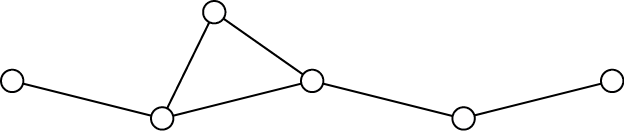
\includegraphics[width=.55\linewidth]{figures/5-path-induce.png}} 
    \vspace{0.2cm}
    \caption{The graph $G$ in \autoref{ex:5-path-induce}. The path on 5 vertices is an induced subgraph of $G$ by removing the highlighted vertex.}
\end{figure}
The facets of its independence complex are
\begin{equation*}
\begin{aligned}
&F_1 = \br{v_1, v_5, v_6}, \\
&F_2 = \br{v_1, v_3, v_5}, \\
&F_3 = \br{v_1, v_4, v_6}, \\
&F_4 = \br{v_2, v_5}, \\
&F_5 = \br{v_2, v_4}
\end{aligned}
\end{equation*}
and a valid solution to the corresponding levelable condition system is given by
$(v_1, v_2, v_3, v_4, v_5, v_6)= (2, 3, 2, 2, 2, 2)$.
\end{example}

While having the path on 5 vertices as an induced subgraph is not a strong enough condition to preclude levelability, we will later prove a result using the idea of an obstruction in \autoref{thm:adjoinment}.


\section{Other observations} 
We used the data from our search to identify families of graphs that are levelable. Below is a summary of some of these results.

\subsection{Cycles and Wheels} \label{subsec:cycles-wheels}
\begin{definition}
A graph $G$ on $n$ vertices is called a \textbf{cycle graph} if its vertices can be labelled  $v_1, \dots, v_n$ such that the edge set is $E(G) = \br{\br{v_i, v_{i+1}} \; | \; i=1, \dots, n-1} \cup \br{\br{v_1, v_n}}$. Then the \textbf{wheel graph} on $n+1$ vertices is the graph with vertex set $V(G) \cup \br{v_{n+1}}$ and edge set $E(G) \cup \br{\br{v_{n+1}, v_i} \; | \; i = 1, \dots, n}$. 
\end{definition}
\begin{figure}[bth]
    \myfloatalign
    \subfloat
    {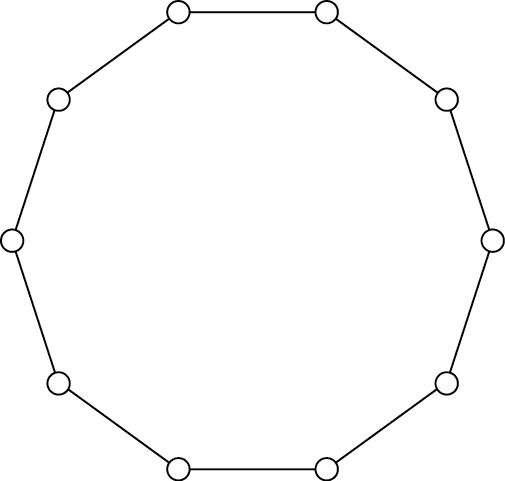
\includegraphics[width=.33\linewidth]{figures/cycle.png}} \qquad 
    \subfloat
    {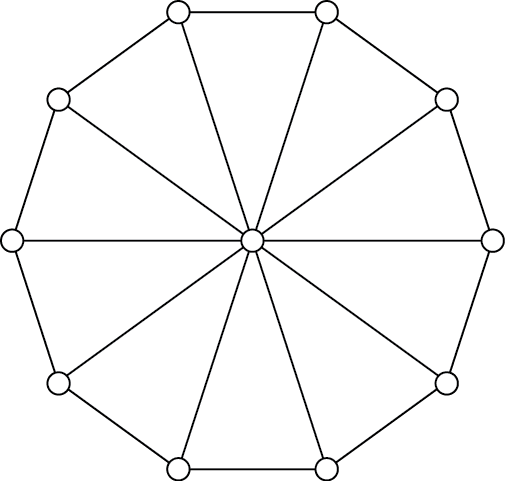
\includegraphics[width=.33\linewidth]{figures/wheel.png}} 
    \caption{The cycle graph on 10 vertices (left), and the wheel graph on 11 vertices (right)}
\end{figure}
Cycle graphs on 8 vertices or greater are not levelable, and the wheel graph on $n$ vertices is levelable if and only if the cycle on $n-1$ vertices is levelable. A general result for cycle graphs is given in \autoref{thm:cycles}. In \autoref{sec:adding-vertices-levelable} and \autoref{sec:adding-vertices-non-levelable} we show that adding a completely connected vertex to a graph does not change whether it is levelable.

\subsection{Long paths are not levelable} \label{subsec:paths} Paths on 5 vertices or greater are not levelable. This result has been generalized to \autoref{thm:graph-partitions}, which uses a proof based on this minimal example.

\subsection{Star graphs are levelable} \label{subsec:star}
\begin{definition} \label{def:star}
A graph $G$ on $n+1$ vertices is called a \textbf{star graph} if its vertices can be labelled $v_0, \dots, v_n$ such that the edge set is $E(G) = \br{\br{v_0, v_i} \; | \; i = 1, \dots, n}$. 
\end{definition}

\begin{figure}[bth]
    \myfloatalign
    {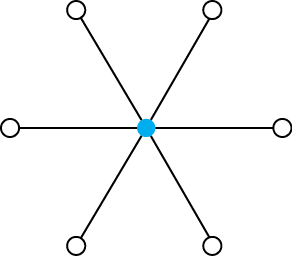
\includegraphics[width=.3\linewidth]{figures/star.png}} 
    \caption{The star graph on 7 vertices. The central vertex $v_0$ is shown in blue.}
\end{figure}

All star graphs are observed to be levelable. A generalization of this result is given in \autoref{thm:complete-multipartite}.
